\pdfoptionpdfminorversion=7
%\documentclass[natbib,twocolumn]{svjour3}
%\documentclass[natbib]{svjour3}
\documentclass[twoside,11pt]{article}
\usepackage{algorithm}
\usepackage{algpseudocode}
\usepackage{float}
\newfloat{algorithm}{t}{lop}
\floatname{algorithm}{\bf Algorithm}
\usepackage[pdftex]{color}
\usepackage{pdfcolmk}
\usepackage[pdftex]{graphicx}
\usepackage{graphicx}
\usepackage{epstopdf}
\usepackage{newtxtext,newtxmath}
\usepackage{bm}
\usepackage{natbib}
\usepackage{setspace}
\PassOptionsToPackage{hyphens}{url}\usepackage{hyperref}

\usepackage[a4paper,head=17mm,headsep=7mm,top=0.8in,left=0.9in,right=0.9in,bottom=0.8in]{geometry}

\bibliographystyle{spbasic}
\usepackage{etoolbox}
\makeatletter
\patchcmd\@combinedblfloats{\box\@outputbox}{\unvbox\@outputbox}{}{\errmessage{\noexpand patch failed}}
\makeatother


\usepackage{marginnote}
\usepackage{amsmath}
\usepackage{amsfonts}
\usepackage{amssymb}
\usepackage{amsbsy}
\pdfminorversion=5

\usepackage{scalerel,stackengine}
\newcommand\pig[1]{\scalerel*[5pt]{\big#1}{%
  \ensurestackMath{\addstackgap[1.5pt]{\big#1}}}}
\newcommand\pigl[1]{\mathopen{\pig{#1}}}
\newcommand\pigr[1]{\mathclose{\pig{#1}}}



\newcommand{\Tinc}  {\tau_\textrm{inc}}
\newcommand{\Tinf}  {\tau_\textrm{inf}}
\newcommand{\Tdeath}{\tau_\textrm{death}}
\newcommand{\Trecm} {\tau_\textrm{recm}}
\newcommand{\Trecs} {\tau_\textrm{recs}}
\newcommand{\Thosp} {\tau_\textrm{hosp}}
\newcommand{\Tint}  {\tau_\textrm{intervention}}

\hypersetup{
    bookmarks=true,         % show bookmarks bar?
    unicode=false,          % non-Latin characters in Acrobat’s bookmarks
    pdftoolbar=true,        % show Acrobat’s toolbar?
    pdfmenubar=true,        % show Acrobat’s menu?
    pdffitwindow=false,     % window fit to page when opened
    pdfstartview={FitH},    % fits the width of the page to the window
    pdftitle={My title},    % title
    pdfauthor={Author},     % author
    pdfsubject={Subject},   % subject of the document
    pdfcreator={Creator},   % creator of the document
    pdfproducer={Producer}, % producer of the document
    pdfkeywords={keyword1, key2, key3}, % list of keywords
    pdfnewwindow=true,      % links in new PDF window
    colorlinks=true,       % false: boxed links; true: colored links
    linkcolor=blue,          % color of internal links (change box color with linkbordercolor)
    citecolor=blue,        % color of links to bibliography
    filecolor=magenta,      % color of file links
    urlcolor=cyan,           % color of external links
}


\newcommand{\E}[1]{\mathbb{E}\left[\, #1 \,\right]}
\newcommand{\benen}{\frac{1}{N} \bmEN\bmEN^\rmT}
\newcommand{\bIenen}{\Big(\bmI-\frac{1}{N} \bmEN\bmEN^\rmT\Big)}

\newcommand{\framedeqX}[1]{
\begin{flushleft}
\fboxrule=0.4mm
\fbox{
\begin{minipage}{0.454\textwidth}
#1
\text{ }
\end{minipage}
}
\end{flushleft}
}








\newcommand {\hpil}{\rightarrow}
\newcommand {\vpil}{\sim}
\newcommand {\D}[2]{\frac{d #1}{d #2}}
\newcommand {\Dd}[2] {\frac{d^2 #1}{d {#2}^2}}
\newcommand {\Dp}[2] {\frac{\partial #1}{\partial #2}}
\newcommand {\Ddp}[2] {\frac{{\partial}^2 #1}{\partial {#2}^2}}
\newcommand {\Ddpp}[2] {\frac{{\partial}^2 #1}{\partial #2^2}}
\newcommand {\del} {\nabla}
\newcommand {\Dj}[3]{\frac{ d_{\scriptstyle{#3}} #1}{d #2}}
\newcommand {\et}{{\scriptscriptstyle \frac{1}{2}}}
\newcommand {\ento}{\frac{1}{2}}
\newcommand {\lp}{\left(}
\newcommand {\rp}{\right)}
\newcommand {\lk}{\left\{ }
\newcommand {\rk}{\right\} }




\newcommand{\rma}{\mathrm{a}}
\newcommand{\rmb}{\mathrm{b}}
\newcommand{\rmc}{\mathrm{c}}
\newcommand{\rmd}{\mathrm{d}}
\newcommand{\rme}{\mathrm{e}}
\newcommand{\rmf}{\mathrm{f}}
\newcommand{\rmg}{\mathrm{g}}
\newcommand{\rmh}{\mathrm{h}}
\newcommand{\rmi}{\mathrm{i}}
\newcommand{\rmj}{\mathrm{j}}
\newcommand{\rmk}{\mathrm{k}}
\newcommand{\rml}{\mathrm{l}}
\newcommand{\rmm}{\mathrm{m}}
\newcommand{\rmn}{\mathrm{n}}
\newcommand{\rmo}{\mathrm{o}}
\newcommand{\rmp}{\mathrm{p}}
\newcommand{\rmq}{\mathrm{q}}
\newcommand{\rmr}{\mathrm{r}}
\newcommand{\rms}{\mathrm{s}}
\newcommand{\rmt}{\mathrm{t}}
\newcommand{\rmu}{\mathrm{u}}
\newcommand{\rmv}{\mathrm{v}}
\newcommand{\rmw}{\mathrm{w}}
\newcommand{\rmx}{\mathrm{x}}
\newcommand{\rmy}{\mathrm{y}}
\newcommand{\rmz}{\mathrm{z}}

\newcommand{\rmA}{\mathrm{A}}
\newcommand{\rmB}{\mathrm{B}}
\newcommand{\rmC}{\mathrm{C}}
\newcommand{\rmD}{\mathrm{D}}
\newcommand{\rmE}{\mathrm{E}}
\newcommand{\rmF}{\mathrm{F}}
\newcommand{\rmG}{\mathrm{G}}
\newcommand{\rmH}{\mathrm{H}}
\newcommand{\rmI}{\mathrm{I}}
\newcommand{\rmJ}{\mathrm{J}}
\newcommand{\rmK}{\mathrm{K}}
\newcommand{\rmL}{\mathrm{L}}
\newcommand{\rmM}{\mathrm{M}}
\newcommand{\rmN}{\mathrm{N}}
\newcommand{\rmO}{\mathrm{O}}
\newcommand{\rmP}{\mathrm{P}}
\newcommand{\rmQ}{\mathrm{Q}}
\newcommand{\rmR}{\mathrm{R}}
\newcommand{\rmS}{\mathrm{S}}
\newcommand{\rmT}{\mathrm{T}}
\newcommand{\rmU}{\mathrm{U}}
\newcommand{\rmV}{\mathrm{V}}
\newcommand{\rmW}{\mathrm{W}}
\newcommand{\rmX}{\mathrm{X}}
\newcommand{\rmY}{\mathrm{Y}}
\newcommand{\rmZ}{\mathrm{Z}}

\newcommand{\calA}{\mathcal{A}}
\newcommand{\calB}{\mathcal{B}}
\newcommand{\calC}{\mathcal{C}}
\newcommand{\calD}{\mathcal{D}}
\newcommand{\calE}{\mathcal{E}}
\newcommand{\calF}{\mathcal{F}}
\newcommand{\calG}{\mathcal{G}}
\newcommand{\calH}{\mathcal{H}}
\newcommand{\calI}{\mathcal{I}}
\newcommand{\calJ}{\mathcal{J}}
\newcommand{\calK}{\mathcal{K}}
\newcommand{\calL}{\mathcal{L}}
\newcommand{\calM}{\mathcal{M}}
\newcommand{\calN}{\mathcal{N}}
\newcommand{\calO}{\mathcal{O}}
\newcommand{\calP}{\mathcal{P}}
\newcommand{\calQ}{\mathcal{Q}}
\newcommand{\calR}{\mathcal{R}}
\newcommand{\calS}{\mathcal{S}}
\newcommand{\calT}{\mathcal{T}}
\newcommand{\calU}{\mathcal{U}}
\newcommand{\calV}{\mathcal{V}}
\newcommand{\calW}{\mathcal{W}}
\newcommand{\calX}{\mathcal{X}}
\newcommand{\calY}{\mathcal{Y}}
\newcommand{\calZ}{\mathcal{Z}}

\newcommand{\bmNull}{{\mathbf{0}}}
\newcommand{\bma}{{\mathbf{a}}}
\newcommand{\bmb}{{\mathbf{b}}}
\newcommand{\bmc}{{\mathbf{c}}}
\newcommand{\bmd}{{\mathbf{d}}}
\newcommand{\hatd}{\hat{\bmd}}
\newcommand{\hatm}{\hat{m}}
\newcommand{\bme}{{\mathbf{e}}}
\newcommand{\bmf}{{\mathbf{f}}}
\newcommand{\bmg}{{\mathbf{g}}}
\newcommand{\bmh}{{\mathbf{h}}}
\newcommand{\bmi}{{\mathbf{i}}}
\newcommand{\bmj}{{\mathbf{j}}}
\newcommand{\bmk}{{\mathbf{k}}}
\newcommand{\bml}{{\mathbf{l}}}
\newcommand{\bmm}{{\mathbf{m}}}
\newcommand{\bmn}{{\mathbf{n}}}
\newcommand{\bmo}{{\mathbf{o}}}
\newcommand{\bmp}{{\mathbf{p}}}
\newcommand{\bmq}{{\mathbf{q}}}
\newcommand{\bmr}{{\mathbf{r}}}
\newcommand{\bms}{{\mathbf{s}}}
\newcommand{\bmt}{{\mathbf{t}}}
\newcommand{\bmu}{{\mathbf{u}}}
\newcommand{\bmv}{{\mathbf{v}}}
\newcommand{\bmw}{{\mathbf{w}}}
\newcommand{\bmx}{{\mathbf{x}}}
\newcommand{\bmy}{{\mathbf{y}}}
\newcommand{\bmz}{{\mathbf{z}}}


\newcommand{\bmA}{{\mathbf{A}}}
\newcommand{\bmB}{{\mathbf{B}}}
\newcommand{\bmC}{{\mathbf{C}}}
\newcommand{\bmD}{{\mathbf{D}}}
\newcommand{\bmE}{{\mathbf{E}}}
\newcommand{\bmF}{{\mathbf{F}}}
\newcommand{\bmG}{{\mathbf{G}}}
\newcommand{\bmH}{{\mathbf{H}}}
\newcommand{\bmI}{{\mathbf{I}}}
\newcommand{\bmJ}{{\mathbf{J}}}
\newcommand{\bmK}{{\mathbf{K}}}
\newcommand{\bmL}{{\mathbf{L}}}
\newcommand{\bmM}{{\mathbf{M}}}
\newcommand{\bmN}{{\mathbf{N}}}
\newcommand{\bmO}{{\mathbf{O}}}
\newcommand{\bmP}{{\mathbf{P}}}
\newcommand{\bmQ}{{\mathbf{Q}}}
\newcommand{\bmR}{{\mathbf{R}}}
\newcommand{\bmS}{{\mathbf{S}}}
\newcommand{\bmT}{{\mathbf{T}}}
\newcommand{\bmU}{{\mathbf{U}}}
\newcommand{\bmV}{{\mathbf{V}}}
\newcommand{\bmW}{{\mathbf{W}}}
\newcommand{\bmX}{{\mathbf{X}}}
\newcommand{\bmY}{{\mathbf{Y}}}
\newcommand{\bmZ}{{\mathbf{Z}}}


\newcommand{\ol}{\overline}

\newcommand{\bmEN}{\mathbf{1}}
\newcommand{\bmSigma}{\boldsymbol{\Sigma}}
\newcommand{\bmOmega}{\boldsymbol{\Omega}}
\newcommand{\bmPi}{\boldsymbol{\Pi}}
\newcommand{\bmLambda}{\boldsymbol{\Lambda}}
\newcommand{\bmdelta}{\boldsymbol{\delta}}
\newcommand{\bmepsilon}{\boldsymbol{\epsilon}}

\newcommand{\red}[1]{{\color{red} #1} }
\newcommand{\blue}[1]{{\color{blue} #1}}
\newcommand{\green}[1]{{\color{green} #1}}



\newcommand{\gradgxfj}{\bmG_{\bmx_j^\rmf}}
\newcommand{\gradgzfj}{\bmG_{\bmz_j^\rmf}}
\newcommand{\gradgzf}{\bmG_{\bmz}}
\newcommand{\gradgqf}{\bmG_\bmq}
\newcommand{\gradgxf}{\bmG_\bmx}


\begin{document}
\setlength{\parskip}{3mm} 

\title{New SEIR with age compartments }
\author{Geir Evensen}
%\institute{G. Evensen \at
%           NORCE (Norwegian Research Center, Bergen, Norway and
%           Nansen Environmental and Remote Sensing Center, Bergen, Norway\\
%           tel.: +47 93 09 09 37\\
%           \email{geir.evensen@norceresearch.no}
%}

\date{Version compiled \today}

\maketitle


\begin{center}
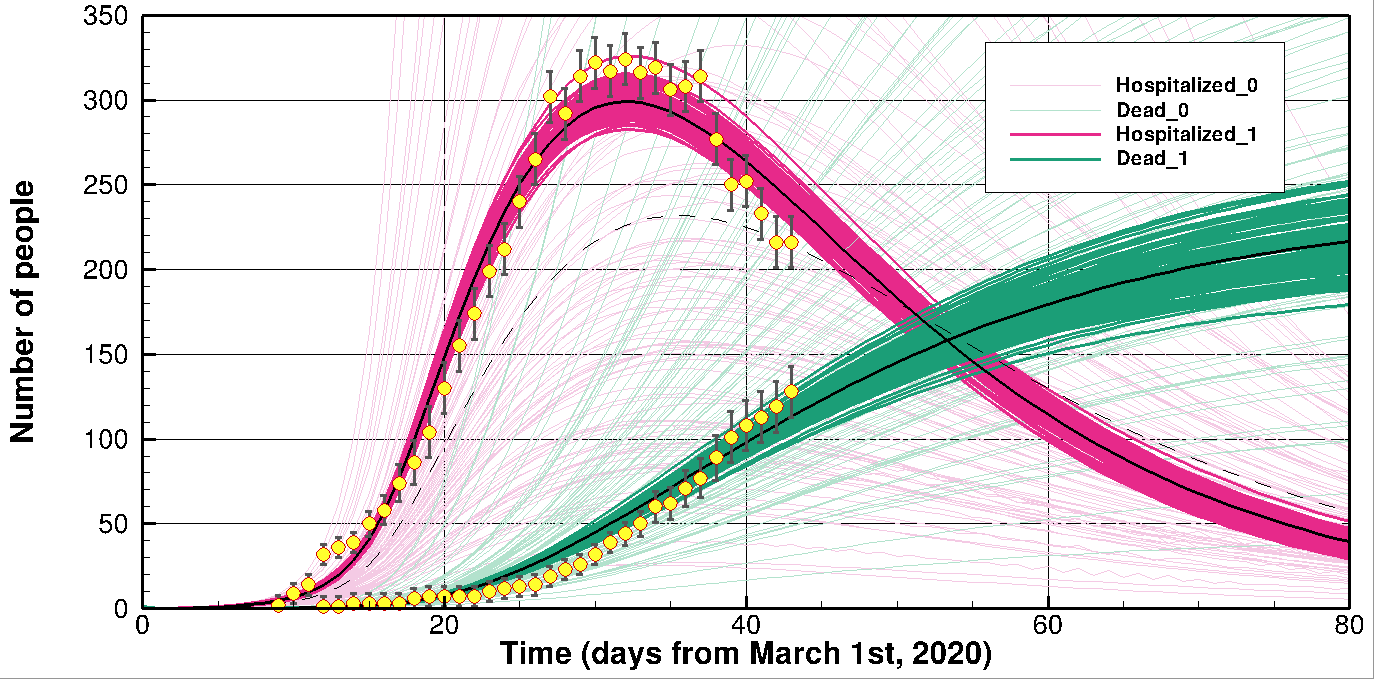
\includegraphics[width=0.99\textwidth]{closed.png} \\
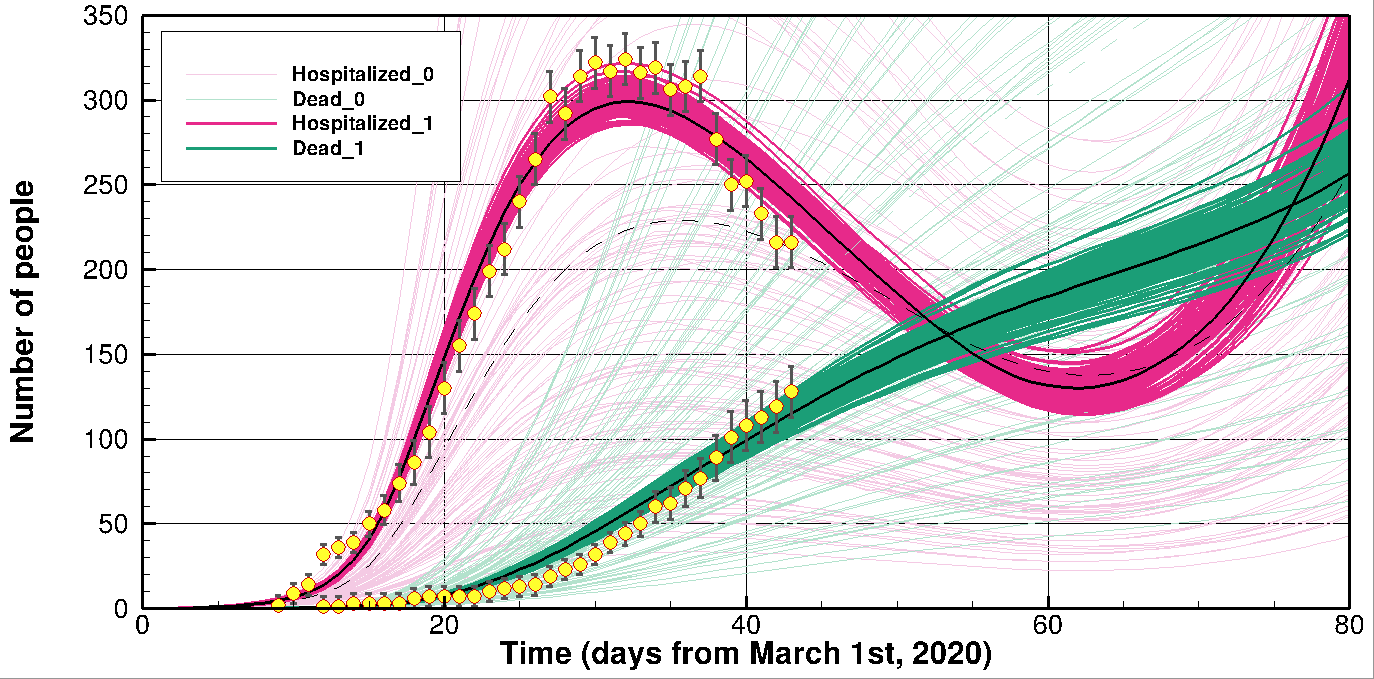
\includegraphics[width=0.99\textwidth]{closed1.png} 
\end{center}

\newpage
\section{SEIR model with agecompartments}
%
\begin{equation}
\begin{cases}
\bmS_1  \hpil &\bmE_1 \hpil \bmI_1 \\
&\vdots \\
\bmS_i  \hpil &\bmE_i \hpil \bmI_i \\
&\vdots \\
\bmS_{n}  \hpil &\bmE_{n} \hpil \bmI_{n} 
\end{cases}
\hpil
\begin{cases}
\bmQ_\rmm                     &  \hpil \bmR_\rmm  \\
\bmQ_\rms    \hpil \bmH_\rms  &  \hpil \bmR_\rms  \\
\bmQ_\rmf    \hpil \bmH_\rmf  &  \hpil \bmD
\end{cases}
\label{eq:}
\end{equation}
%
The model equations are as follows:
%
\begin{align}
\Dp{\bmS_i}{t}    &=   -\frac{1}{\Tinf} \bigg(\sum_{j=1}^n R_{ij}(t)\,\bmI_j\bigg) \, \bmS_i                           \label{eq:Si} \\
\Dp{\bmE_i}{t}    &=    \frac{1}{\Tinf} \bigg(\sum_{j=1}^n R_{ij}(t)\,\bmI_j\bigg) \, \bmS_i - \frac{1}{\Tinc}\, \bmE_i      \label{eq:Ei} \\
\Dp{\bmI_i}{t}    &=    \frac{1}{\Tinc}  \, \bmE_i          - \frac{1}{\Tinf}  \, \bmI_i                                     \label{eq:Ii} \\
\Dp{\bmQ_\rmm}{t} &=    \sum_{i=1}^n\frac{p_\rmm^i}{\Tinf} \, \bmI_i          - (1/\Trecm)  \, \bmQ_\rmm         \label{eq:Sm} \\
\Dp{\bmQ_\rms}{t} &=    \sum_{i=1}^n\frac{p_\rms^i}{\Tinf} \, \bmI_i          - (1/\Thosp)  \, \bmQ_\rms         \label{eq:Sh} \\
\Dp{\bmQ_\rmf}{t} &=    \sum_{i=1}^n\frac{p_\rmf^i}{\Tinf} \, \bmI_i          - (1/\Thosp)  \, \bmQ_\rmf          \label{eq:Sdead} \\
\Dp{\bmH_\rms}{t} &=    (1/\Thosp)     \, \bmQ_\rms     - (1/\Trecs)  \, \bmH_\rms         \label{eq:Shos} \\
\Dp{\bmH_\rmf}{t} &=    (1/\Thosp)     \, \bmQ_\rmf     - (1/\Tdeath) \, \bmH_\rmf         \label{eq:Fhos} \\
\Dp{\bmR_\rmm }{t}&=    (1/\Trecm)     \, \bmQ_\rmm                                        \label{eq:Rm} \\
\Dp{\bmR_\rms}{t} &=    (1/\Trecs)     \, \bmH_\rms                                        \label{eq:E} \\
\Dp{\bmD     }{t} &=    (1/\Tdeath)    \, \bmH_\rmf                                        \label{eq:E} 
\end{align}


\clearpage
\newpage
\section{Some model parameters}
\begin{table}[htb]
\begin{center}
\small
\tabcolsep=3.5pt
\begin{tabular}{lccccccccccc}
\hline
 Age group & 1      & 2      & 3      & 4      & 5      & 6      & 7      & 8      & 9      & 10     & 11      \\
 Age range & 0--5   & 6--12  & 13--19 & 20--29 & 30--39 & 40--49 & 50--59 & 60--69 & 70--79 & 80--89 & 90--105 \\
 Population& 351159 & 451246 & 446344 & 711752 & 730547 & 723663 & 703830 & 582495 & 435834 & 185480 & 45230   \\
 P--mild   & 1.0000 & 1.0000 & 1.0000 & 1.0000 & 1.0000 & 0.9640 & 0.9185 & 0.9210 & 0.8900 & 0.9070 &  0.9120 \\
 P--severe & 0.0000 & 0.0000 & 0.0000 & 0.0000 & 0.0000 & 0.0360 & 0.0720 & 0.0600 & 0.0720 & 0.0360 &  0.0120 \\
 P--fatal  & 0.0000 & 0.0000 & 0.0000 & 0.0000 & 0.0000 & 0.0000 & 0.0095 & 0.0190 & 0.0380 & 0.0570 &  0.0760 \\
\hline
\end{tabular}
\end{center}
\caption{
The population numbers are obtained from SSB and are accurate. The total Norwegan population is 5367580.
The P numbers indicate the fraction of sick people in an age group ending up with mild symptons, severe symptons (hospitalized),
and fatal infection (hospitalized and then dead).
\textbf{These numbers are currently defined in m\_pfactor.F90 but will later be read from a file.}
\label{tab:age}}
\end{table}
%

\begin{table}[htb]
\begin{center}
\tabcolsep=3.5pt
\begin{tabular}{c|ccccccccccc}
\hline
 Age group & 1      & 2      & 3      & 4      & 5      & 6      & 7      & 8      & 9      & 10     & 11      \\
\hline
    1      & \bf 3.80   & 2.00   &   2.00 &     1.50 &     1.50  &    1.10  &    0.80  &    0.80  &    0.80  &    0.80 &     0.80  \\
    2      & 2.00   & \bf 3.80   &   2.00 &     1.50 &     1.50  &    1.50  &    0.80  &    0.80  &    0.80  &    0.80 &     0.80  \\
    3      & 2.00   & 2.00   &  \bf  1.00 &     1.00 &     0.90  &    0.80  &    0.80  &    0.80  &    0.80  &    0.80 &     0.80  \\
    4      & 1.50   & 1.50   &   1.00 &   \bf   0.80 &     0.80  &    0.80  &    0.80  &    0.80  &    0.80  &    0.80 &     0.80  \\
    5      & 1.50   & 1.50   &   0.90 &     0.80 &  \bf    0.80  &    0.80  &    0.80  &    0.80  &    0.80  &    0.80 &     0.80  \\
    6      & 1.10   & 1.50   &   0.80 &     0.80 &     0.80  &  \bf   0.80  &    0.80  &    0.80  &    0.80  &    0.80 &     0.80  \\
    7      & 0.80   & 0.80   &   0.80 &     0.80 &     0.80  &    0.80  &  \bf   0.80  &    0.80  &    0.80  &    0.80 &     0.80  \\
    8      & 0.80   & 0.80   &   0.80 &     0.80 &     0.80  &    0.80  &    0.80  & \bf    0.80  &    0.80  &    0.80 &     0.80  \\
    9      & 0.80   & 0.80   &   0.80 &     0.80 &     0.80  &    0.80  &    0.80  &    0.80  &  \bf   0.80  &    0.80 &     0.80  \\
    10     & 0.80   & 0.80   &   0.80 &     0.80 &     0.80  &    0.80  &    0.80  &    0.80  &    0.80  & \bf    0.80 &     0.80  \\
    11     & 0.80   & 0.80   &   0.80 &     0.80 &     0.80  &    0.80  &    0.80  &    0.80  &    0.80  &    0.80 &  \bf    0.80  \\
\hline
\end{tabular}
\end{center}
\caption{The $R$ matrix allows for using different transmission factors in between different age groups.
This matrix was used after opening up children schools and kinder gardens. On the diagonal the value gives the 
transmission of desease within the same age group. The off-diagonal terms are the transmissions between age groups.
Here it is assumed that open kinder gardens and schools leads to ``normal'' transmission within these groups $R=3.8$.
We also assume that there are increased transmission between parent groups and children.
\textbf{These numbers are currently defined in m\_Rmatrix.F90 but will later be read from a file.}
\label{tab:R}}
\end{table}
%



%
\subsection{Model paramters}
\begin{center}
\small
\begin{tabular}{lll}
\hline
$I_0    = 50.0                $&    Initial infectious                                  \\
$R_0    = 5.0                 $&    Basic Reproduction Number                           \\
$\Tinf  = 2.9                 $&    Infections time                                     \\
$\Tinc  = 5.2                 $&    Incubation period                                   \\
$\Trecm = 11.1                $&    Recovery time mild cases (11.1)                     \\
$\Trecs = 15.0                $&    Recovery time severe cases Length of hospital stay  \\
$\Thosp = 5.0                 $&    Time to hospitalization.                            \\
$\Tdeath = 15.0               $&    Days to death                                       \\
$p_\rmf = 0.006               $&    Case fatality rate                                  \\
$p_\rms = 0.012               $&    Hospitalization rate \% for severe cases            \\
$R(t)   = 0.63                $&    Basic Reproduction Number during intervention       \\
\hline
\end{tabular}
\end{center}
%
%
\subsection{Diagnostic variables}
\begin{center}
\begin{tabular}{ll}
\hline
Number of hospitelized & $N(\bmH_\rms + \bmH_\rmf)$ \\
Number of recovered    & $N(\bmR_\rmm+\bmR_\rms)$ \\
Number of deaths       & $N\bmD$ \\
Number of exposed      & $N\sum \bmE_i$ \\
Number of infectious   & $N\sum \bmI_i$ \\
Number of susceptible  & $N\sum \bmS_i$ \\
\hline
\end{tabular}
\end{center}



\bibliography{geir,geirres}

\end{document}
